% Generated by scratchpad/restructure.py -- ten supporting sections moved
% out of Chapter 5. Content is verbatim; only three subsection headings
% were promoted to sections because they lost their parent.
\section{Ground-Truth Anchoring}

Cross-view consistency compares two predictions to each other and is in principle insensitive to errors shared by both views, so we anchor it against ground truth. World-transformed ground truth from different cameras agrees to 0.00 mm, which confirms that the reference frame is view-independent. We find that canonical cross-view distance correlates with true prediction error at a Spearman coefficient of $+0.601$ over 1566 frames, against $+0.188$ for the raw distance. This suggests that canonicalization makes cross-view consistency a substantially stronger proxy for actual error.

\section{Reliability Under Controlled Degradation}

We applied five physically motivated corruptions at graduated severities over a sweep of 2240 records. Reliability tracks induced error at a Spearman coefficient of $-0.813$, joint dropout produces abstention in 100 percent of cases, and clean frames produce abstention in none. Identity-severity controls reproduced the clean baseline exactly. Figure \ref{fig:degradation} shows the relationship for each operator.

\begin{figure}[htbp]
\centering
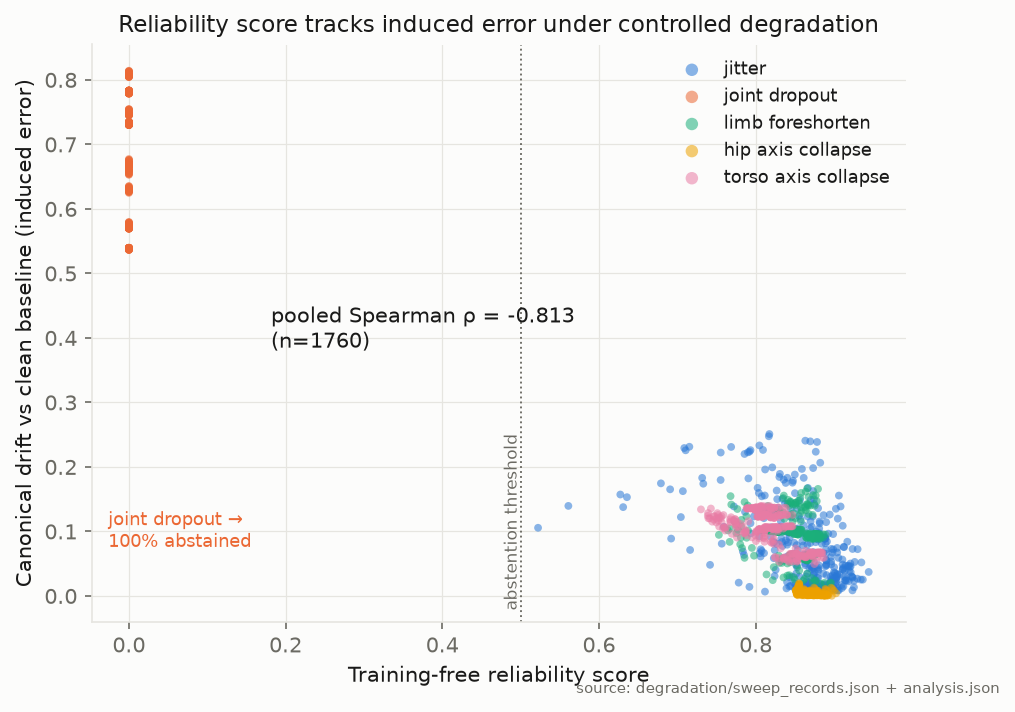
\includegraphics[width=0.72\textwidth]{images/fig_degradation.png}
\caption{Reliability against induced error for five corruption operators}
\label{fig:degradation}
\end{figure}

\section{Multi-Scale Canonicalization}

Per-limb frames improve every one of the twenty-nine pairs, by 37.1 percent on the development pair and by 36.4 percent on average over held-out pairs. The improvement is not an artifact of reduced degrees of freedom, since the multi-scale distance retains its correlation with ground-truth error at $+0.610$ against $+0.601$ for the global frame. Figure \ref{fig:multiscale} shows the per-pair gain.

\begin{figure}[htbp]
\centering
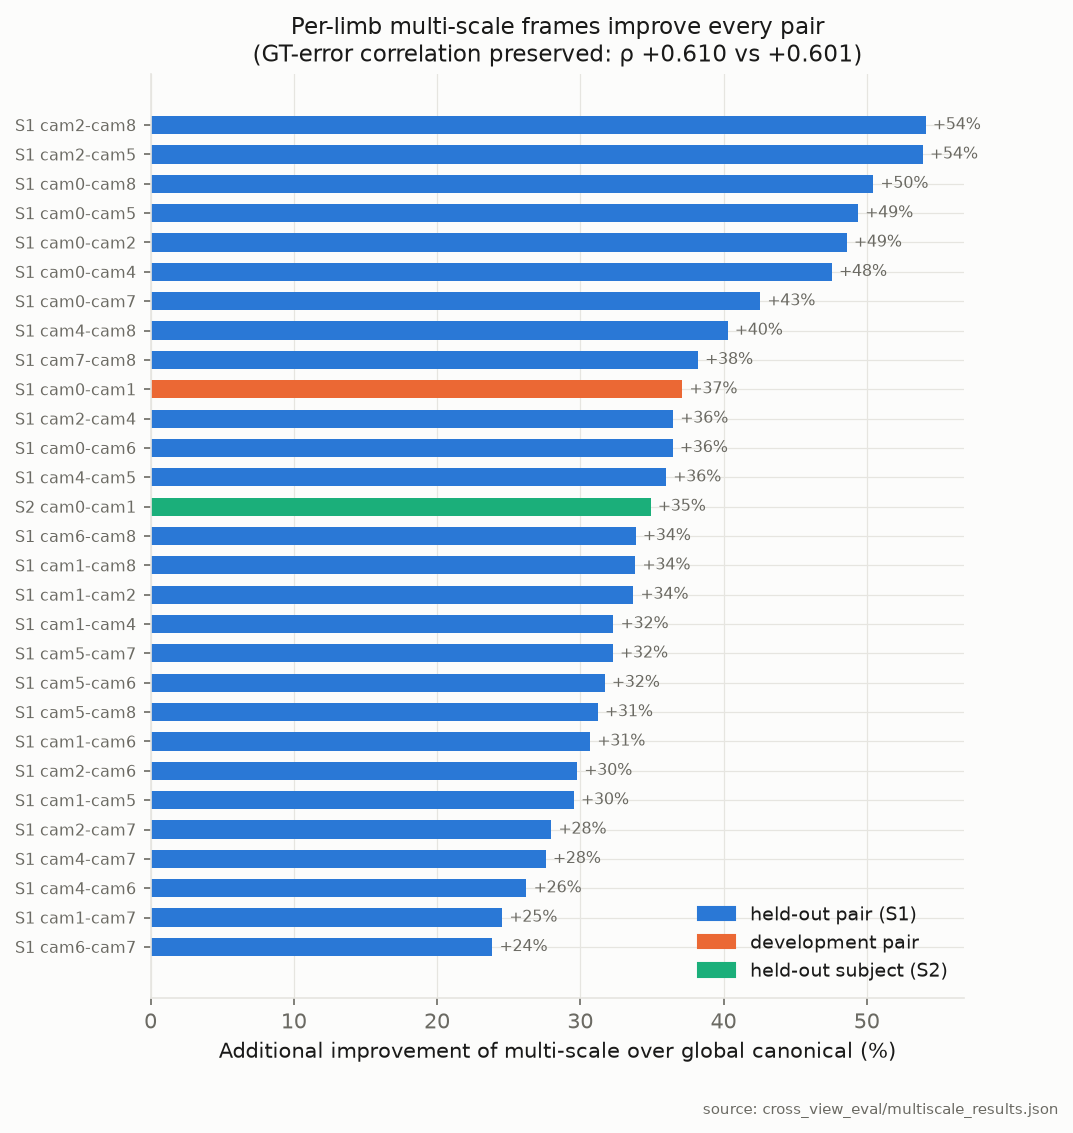
\includegraphics[width=0.95\textwidth]{images/fig_multiscale.png}
\caption{Additional improvement of multi-scale over global canonicalization}
\label{fig:multiscale}
\end{figure}

\section{Multi-View Fusion and a Negative Result on Selection}

Fusion improves on an arbitrary single view in all four conditions, by 23.7 and 10.6 percent on subject S1 under static and dynamic motion and by 10.2 and 8.2 percent on subject S2. Because averaging does not require knowing which view is best, the result is robust. Figure \ref{fig:fusion} shows how the gain scales with the number of available cameras while the single-view baseline stays flat.

Selection, by contrast, does not survive scrutiny. We initially measured a 33.8 percent gain from selecting the most reliable view, but we find this to be an artifact: on static footage the score selects the same camera in every frame, and the gain arises from that constant choice combined with a large spread of per-view error. On dynamic sequences the selected view's true-error rank is 4.78 of 8 on subject S1 against a chance expectation of 4.5, and 3.67 on subject S2, straddling chance in opposite directions. We therefore withdraw the claim.

\begin{figure}[htbp]
\centering
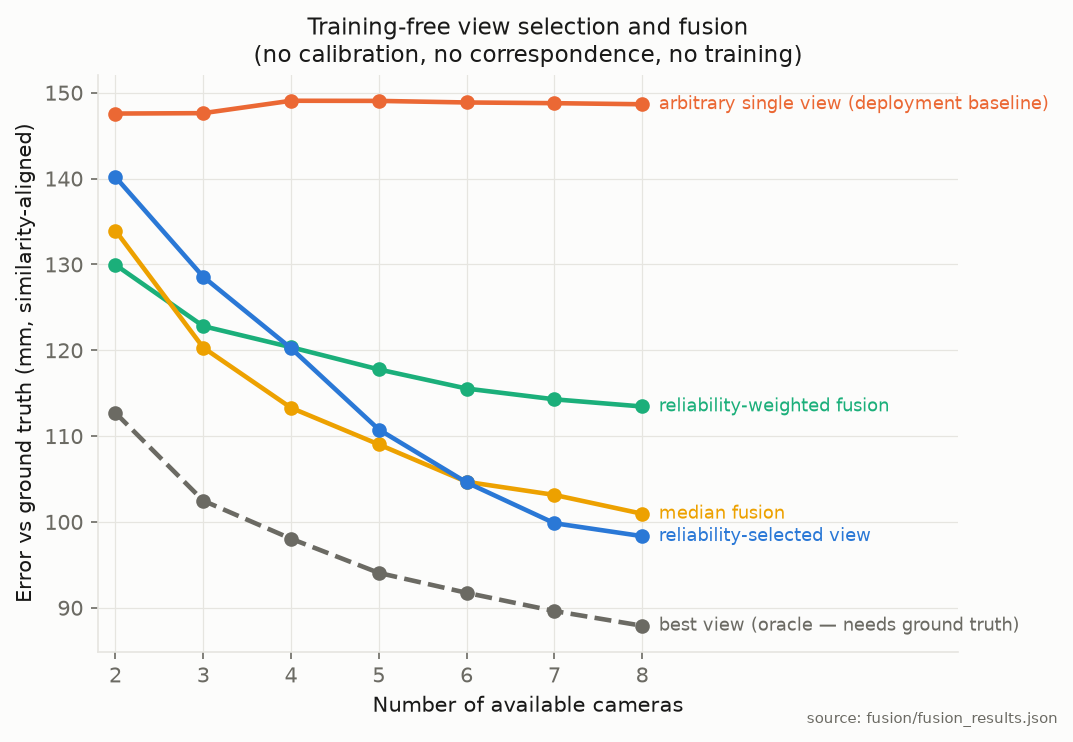
\includegraphics[width=0.75\textwidth]{images/fig_fusion.png}
\caption{Error against number of available cameras for each strategy}
\label{fig:fusion}
\end{figure}

\section{Orientation or Translation?}
\label{sec:translation}

The two methods do not place their poses at the same origin. Ours is root-centred, putting joint 0 at the origin; the template baseline is centroid-centred, because the Kabsch fit subtracts the mean of the point set. Centroid-centring averages seventeen joints where root-centring relies on one, so some of the reported advantage may be steadier translation rather than better orientation. We pre-registered the separation and ran the two-by-two, changing only where the output is centred and leaving both estimators untouched.

\begin{table}[htbp]
\centering
\caption[Orientation or translation]{Mean cross-view distance in millimetres under each centring, on the same 180 pairs. Only the origin of the output changes; the rotation estimates are unaltered.}
\label{tab:translation}
{\fontsize{10}{12}\selectfont
\begin{tabular}{llrr}
\hline
\textbf{Backbone} & \textbf{Method} & \textbf{Root-centred} & \textbf{Centroid-centred} \\
\hline
MotionAGFormer-XS & anatomical & 75.32 & 75.85 \\
                  & template   & 59.96 & \textbf{53.03} \\
\hline
MotionBERT        & anatomical & 60.09 & 60.78 \\
                  & template   & 56.93 & \textbf{51.27} \\
\hline
\end{tabular}}
\end{table}

Three things follow. \textbf{The baseline wins under every centring on both backbones}, with intervals excluding zero in all four cases, so the result of Section \ref{sec:template} is not an artifact of the mismatch. \textbf{Orientation accounts for the majority of the gap and translation for a minority the two backbones do not agree on}: comparing like with like gives 19.1 and 6.3 mm against the 22.3 and 8.8 reported, putting translation at 14 percent of the advantage on the first backbone and 28 on the second. That is a factor of two between two estimators of the same pose on the same frames, so the share is not a stable quantity and we do not report a single figure for it. \textbf{And the magnitude is centring-dependent in a way worth stating plainly.} Under the centring least favourable to the baseline, both methods root-centred, the gap on MotionBERT falls from 8.8 mm to 3.2, an interval of $[-4.8, -1.5]$. The direction of the result is robust; its size is not, and a reader comparing these methods should know which convention produced which number.

The asymmetry has a simple cause. Centroid-centring improves the template by 6.9 and 5.7 mm because its rotation was fitted under exactly that centring, so the two agree. It makes the anatomical frame slightly \emph{worse}, by 0.5 and 0.7 mm, because that frame is constructed about the root and re-centring it elsewhere is inconsistent with its own definition. Each method is best served by the origin it was built for, which is why the mixed comparison in Section \ref{sec:template} --- each method in its natural form --- remains the one a practitioner would face.

\section{Does the Baseline Have a Failure Mode? It Does Not}
\label{sec:templateaction}

One defence of an anatomically-defined frame remains available in principle. The template is a single fixed near-standing skeleton, and 180 pairs drawn from fifteen largely upright actions may simply not contain the poses where aligning everything onto one reference breaks down. We pre-registered the breakdown, with the reading fixed in advance that if the baseline never loses then the anatomical frame has no regime of its own and this report should say so rather than leave a niche implied.

\textbf{The baseline wins on all fifteen actions, on both backbones.} The margin ranges from 12.4 to 245.9 mm on the first backbone and 10.7 to 29.7 on the second. There is no action, and therefore no identified pose regime within Human3.6M, in which the anatomical construction is preferable.

The largest margin locates the point precisely. SittingDown is the action on which our frame fails worst throughout this report, at 335.0 mm on the thirteen non-constructor joints, and it is exactly where the template helps most, reaching 89.1 mm. The failure Section \ref{sec:h36mcv} attributes to the estimator degrading on a foreshortened torso is not, on this evidence, an estimator failure that any frame must inherit: a different training-free frame recovers most of it from the same predictions. Walking, the action closest to a standing template and the one where a fixed reference should have been most favoured, shows the \emph{smallest} margin at 12.4 mm --- the opposite of the pattern that would have named a regime for us.

We state the consequence rather than leave it to be inferred. Within the scope of this evaluation, the two-vector anatomical frame is not preferable to Kabsch alignment against a fixed skeleton for any action, at any centring, under any of the three templates tested. What the anatomical construction retains is that it is defined by named anatomical landmarks and so yields a frame with an interpretable orientation, where the template's frame is whatever the reference skeleton happened to be pointing at; nothing in this report measures whether that interpretability is worth its cost.

\section{Two Further Ablations of That Baseline}
\label{sec:templateablation}

Two objections to the comparison arise immediately and neither is answered by the experiment that produced it. Both were pre-registered and run.

\textbf{The win does not depend on our own canonicalization.} The template above is the mean \emph{canonical} MPI pose, and those poses were aligned by the construction the baseline defeats, so the baseline might be inheriting something from its opponent. We rebuilt it two ways that cannot: from a single arbitrary raw MPI prediction with no canonicalization anywhere in its construction, and from a synthetic standing figure assembled from median bone lengths along fixed anatomical directions, which uses no pose data at all. The baseline wins under all three on both backbones. On the first backbone the paired difference is $-22.3$, $-21.5$ and $-19.9$ mm for the canonical, raw and synthetic templates, and on the second $-8.8$, $-8.0$ and $-6.4$ mm, every interval excluding zero. A figure built from nothing but median bone lengths still beats the anatomical frame, which makes the result stronger than when it was first reported rather than weaker.

\textbf{The boundary analysis does not translate into a better fit set, and the reason is instructive.} Section \ref{sec:radial} shows that joints beyond a hinge disagree far more across views than joints rigid with the torso, which suggests that a least-squares fit over all seventeen is being dragged by its worst-determined points. We predicted before running that fitting the rotation on the nine torso-rigid joints and scoring on the eight articulated ones would beat fitting on all seventeen. \textbf{It does not.} Fitting on all seventeen gives 67.6 and 66.6 mm on the two backbones against 96.3 and 91.8 for the torso-rigid fit, so the prediction fails by roughly 25 mm in the wrong direction.

Two explanations are available and we have not separated them, so we name both rather than assert the one that suits us.

The first is the overlap this report keeps meeting. When the fit uses all seventeen joints it includes the eight being scored, so it is partly aligning the very quantity the metric then measures, where the torso-rigid fit is disjoint from the scored set and enjoys no such advantage. On that reading the two numbers are not comparable as a test of fit sets at all, and the 67.6 mm figure is optimistically biased exactly as Section \ref{sec:circularity} describes for the per-limb frames.

The second is our own principle applied one level up. The nine torso-rigid joints lie close to a single plane, because the limbs are what give a skeleton its anterior-posterior extent, and a near-planar point set determines rotation about its in-plane axes poorly for the same lever-arm reason a short axis does. Equation \eqref{eq:theta} concerns a direction read from two joints, but the mechanism carries: a fit has little to work with along the direction in which its points barely spread. On that reading the torso-rigid set is simply an ill-conditioned one to fit from, and the overlap is incidental.

Both predict the failure we observed and this experiment cannot distinguish them. Elsewhere in this report we rejected the foreshortening account of SittingDown and the spurious-correlation account of the bone-length signal by testing the alternative, and we do not have the equivalent here; Section \ref{sec:future} states the test that would settle it. What the disjoint arrangement does give is the cleanest single comparison in this report, since no joint used to fit is scored: on the eight articulated joints the template reaches 96.3 and 91.8 mm against the anatomical frame's 121.9 and 97.0. The baseline still wins, though on the second backbone the margin narrows from 8.8 mm to 5.2 once the fit can no longer see what is being scored.

Two things about the non-constructor recomputation are worth stating because they are not obvious. Excluding those joints raises the canonical distance, since the pinned joints were dragging it down, but it also raises the raw distance from 320.4 to 372.7 mm, because the hips and thorax are among the joints two cameras disagree about least before canonicalization. The improvement is a ratio of the two, and we did not predict which term would move further; the pre-registration in \texttt{thesis\_artifacts/noncon/} records that explicitly and forbids the verification from checking whether the figure fell. It fell by 1.8 points on one backbone and 1.7 on the other, which is the size of the artifact rather than its refutation.

\textbf{That percentage is not the one the two column means give, and the difference is a convention rather than an error.} Every improvement figure in this report is the mean over camera pairs of each pair's own percentage improvement. Forming the ratio from the aggregate means instead would give 76.5 percent here and 81.0 percent on the second backbone. We use the per-pair mean throughout because it weights each pair equally, whereas the ratio of means lets the widest-baseline pairs, which have the most to gain, dominate the figure. The per-pair convention is the lower of the two in every case we report, so the choice is conservative; but a reader dividing the table entries will not reproduce the headline, and should know why. The same distinction governs the oracle-gap figures below and the action-balanced accuracy of Section \ref{sec:h36m}. A cluster bootstrap that resamples whole subject and action groups, rather than individual pairs, places the improvement in the interval $[+69.8, +77.2]$ percent. The clustering matters here: the six pairs of a group are formed from the same four camera streams of the same motion, so resampling pairs individually would treat 180 dependent observations as independent and return an interval that is too narrow. The interval excludes the 32.4 percent obtained on MPI-INF-3DHP by a wide margin, so the difference between the two datasets is not attributable to sampling. The per-frame Procrustes oracle reaches 51.3 mm, so canonicalization closes 90.5 percent of the gap between an arbitrary pair of viewpoints and the best a rotation can achieve. As above, that is the mean over pairs of each pair's own gap-closed fraction; the ratio of the column means would give 91.1 percent, and 96.1 rather than 94.5 on the second backbone. The body frame is well conditioned on every frame evaluated, giving a validity rate of 100 percent.

That comparison invites an obvious question, which we answer here rather than leave standing: if the oracle is better, why not simply use it. The oracle aligns two poses to each other, so it requires both of them at once, and what it returns is a relative alignment rather than a representation. It cannot canonicalize a single pose, because there is nothing to align that pose to; it cannot run before a comparison exists, so it cannot be used to index, store or stream; and with $N$ cameras it must be recomputed for each of the $N(N-1)/2$ pairs, whereas a body frame is computed once per pose and every pair is then comparable by construction. The oracle is included as a floor on what any rotation can achieve, not as a competing method. The relevant claim is that a construction which sees one pose at a time recovers most of what a construction that sees both can do.

\begin{table}[htbp]
\centering
\caption{Cross-view canonicalization on Human3.6M, 180 held-out camera pairs.}
\label{tab:h36mcv}
\begin{tabular}{lrr}
\hline
\textbf{Quantity} & \textbf{Human3.6M} & \textbf{MPI-INF-3DHP} \\
\hline
Camera pairs & 180 & 29 \\
Pairs held out & 180 & 27 \\
Raw cross-view distance & 320.4 mm & --- \\
Canonical cross-view distance & 75.3 mm & --- \\
Procrustes oracle & 51.3 mm & --- \\
Mean improvement & +74.1\% & +32.4\% \\
95\% CI, clustered by group & $[+69.8, +77.2]$ & --- \\
Median improvement & +81.6\% & --- \\
Pairs improved & 179 / 180 & 27 / 27 \\
Oracle gap closed & 90.5\% & --- \\
Canonicalization validity & 100.0\% & --- \\
\hline
\end{tabular}
\end{table}

\begin{figure}[htbp]
\centering
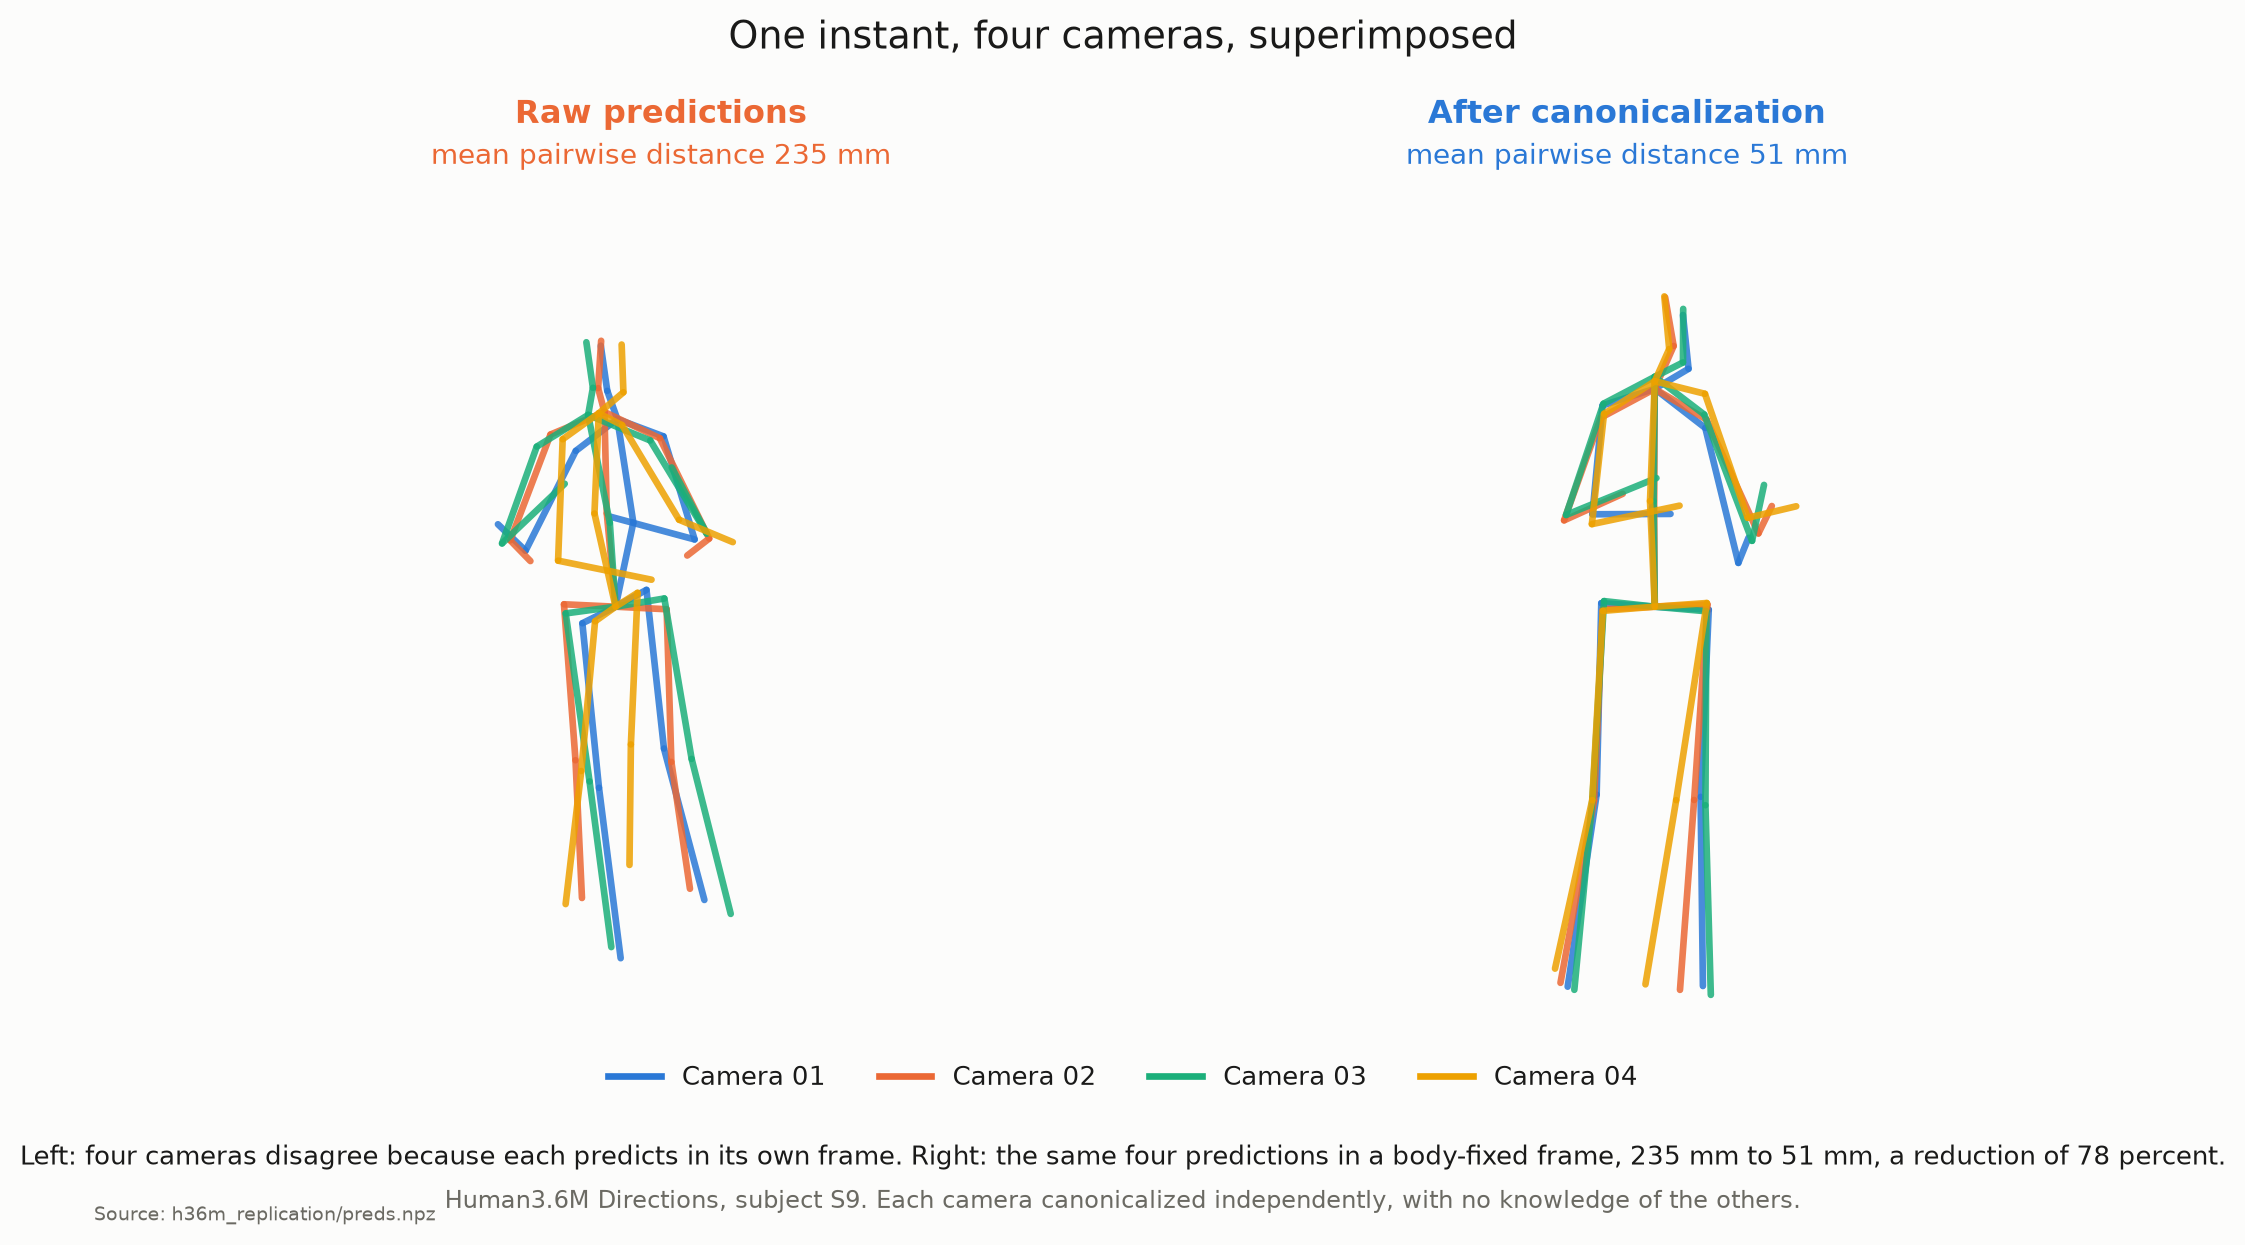
\includegraphics[width=\textwidth]{images/fig_h36m_explainer.png}
\caption[One instant of Human3.6M seen by four synchronized cameras, superimposed]{One instant of Human3.6M seen by four synchronized cameras, superimposed. Left: the four raw predictions, which disagree because each is expressed in the frame of its own camera. Right: the same four predictions after canonicalization, each computed independently and without knowledge of the others.}
\label{fig:h36mexplain}
\end{figure}

\begin{figure}[htbp]
\centering
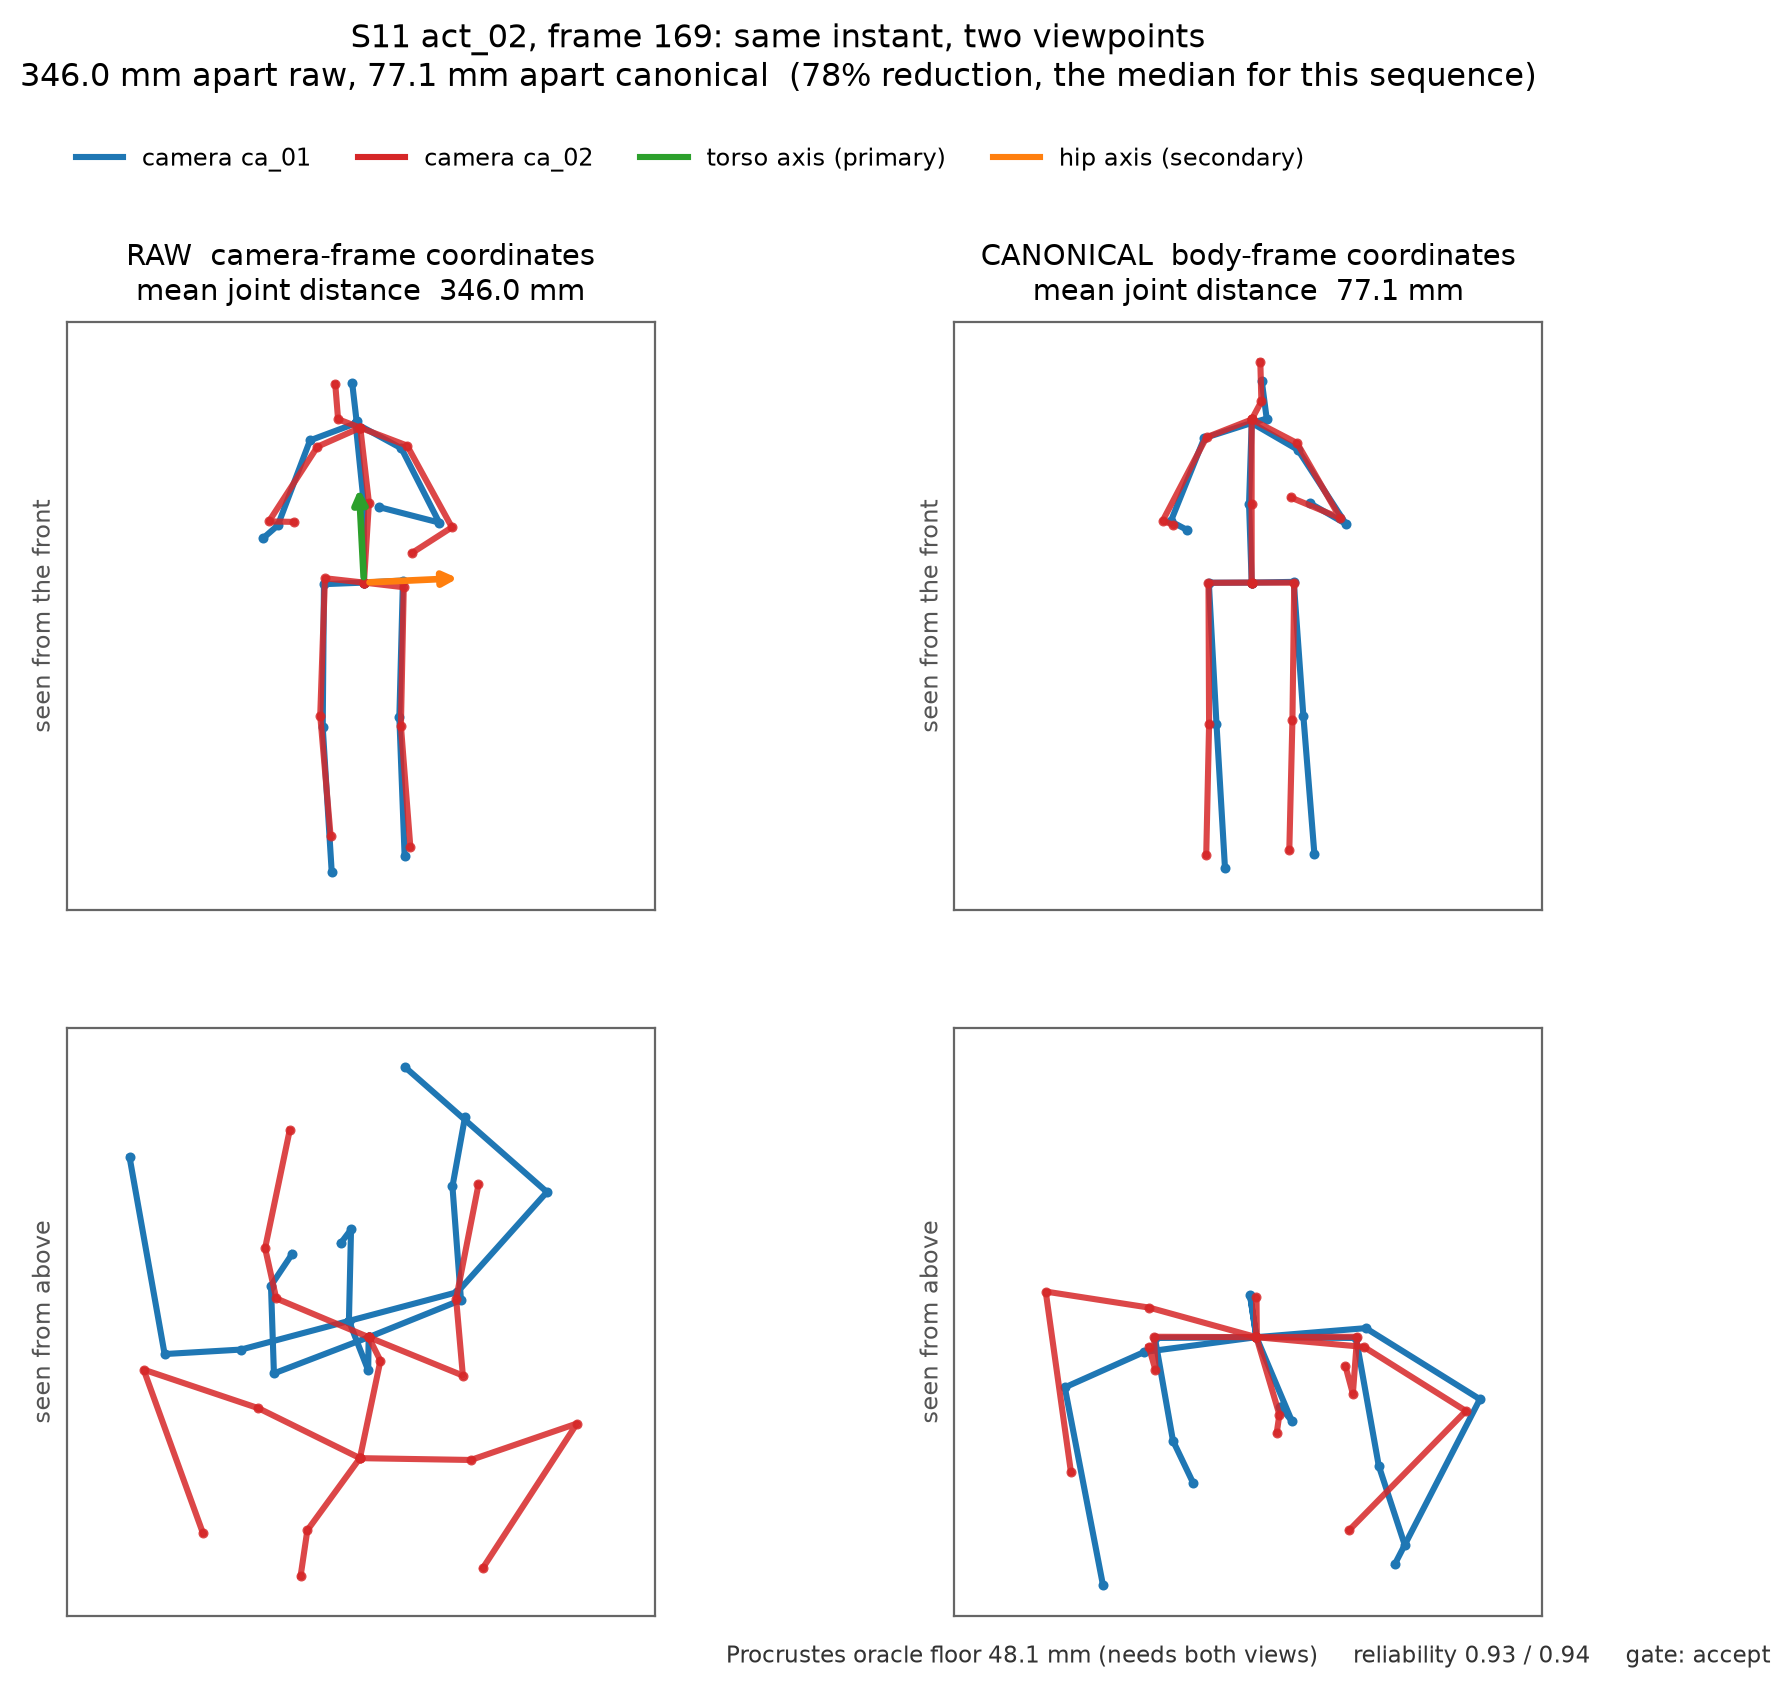
\includegraphics[width=0.78\textwidth]{images/fig_twoview.png}
\caption[One camera pair in detail]{One camera pair in detail, at the frame whose improvement is the median for its sequence rather than the most favourable. The lower row is the same data seen from above, and it is included because it is where the disagreement actually lives: two cameras of one instant differ mainly in azimuth, which a frontal projection almost entirely conceals. Both columns of a row are drawn to the same scale. The oracle floor and the reliability gate are shown because the method reaches neither perfection nor the floor, and a figure that omitted them would suggest otherwise.}
\label{fig:twoview}
\end{figure}

Figure \ref{fig:h36mexplain} shows what the aggregate hides. Four cameras observing one instant produce four sets of coordinates that visibly disagree, and the same four predictions in a body-fixed frame very nearly coincide, at 235 mm and 51 mm respectively on that frame. No camera has any knowledge of the others at any point.

\begin{figure}[htbp]
\centering
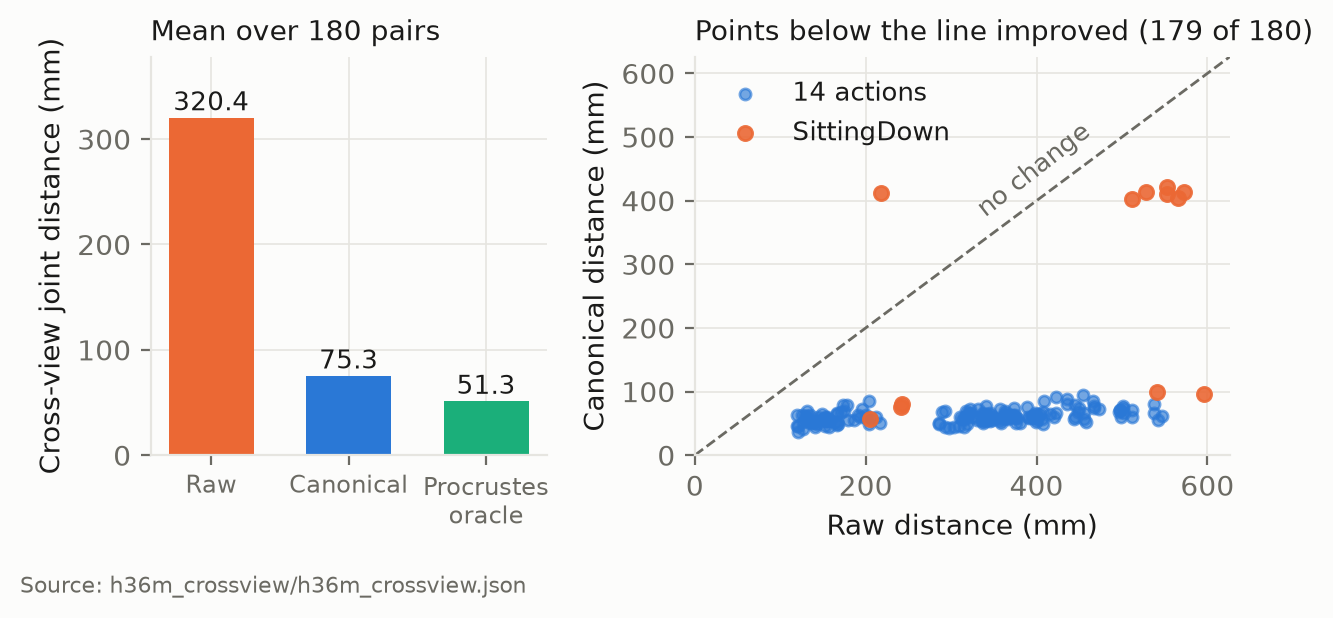
\includegraphics[width=\textwidth]{images/fig_h36m_distances.png}
\caption[Cross-view distance on Human3.6M]{Cross-view distance on Human3.6M. Left: means over all 180 held-out pairs. Right: every pair individually, with the diagonal marking no change. Canonical distance collapses to a narrow band irrespective of how far apart the two raw predictions were, except on SittingDown.}
\label{fig:h36mdist}
\end{figure}

The right panel of Figure \ref{fig:h36mdist} shows why the mean is not carried by a few easy pairs. Raw distance varies from roughly 120 mm to 600 mm across pairs, and canonical distance is almost flat across that range at between 40 mm and 100 mm. The reduction therefore does not depend on how far apart the two viewpoints happened to be, which is the behaviour a frame construction should exhibit if it is genuinely removing viewpoint rather than partially compensating for it.

The result holds on both subjects. Subject S11 improves on all ninety of its pairs, from 21.2 percent to 89.7 percent, and subject S9 improves on eighty-nine of ninety. Fourteen of the fifteen actions improve on every one of their twelve pairs, with canonical distances between 45.3 mm and 79.6 mm, as Figure \ref{fig:h36macts} shows.

\begin{figure}[htbp]
\centering
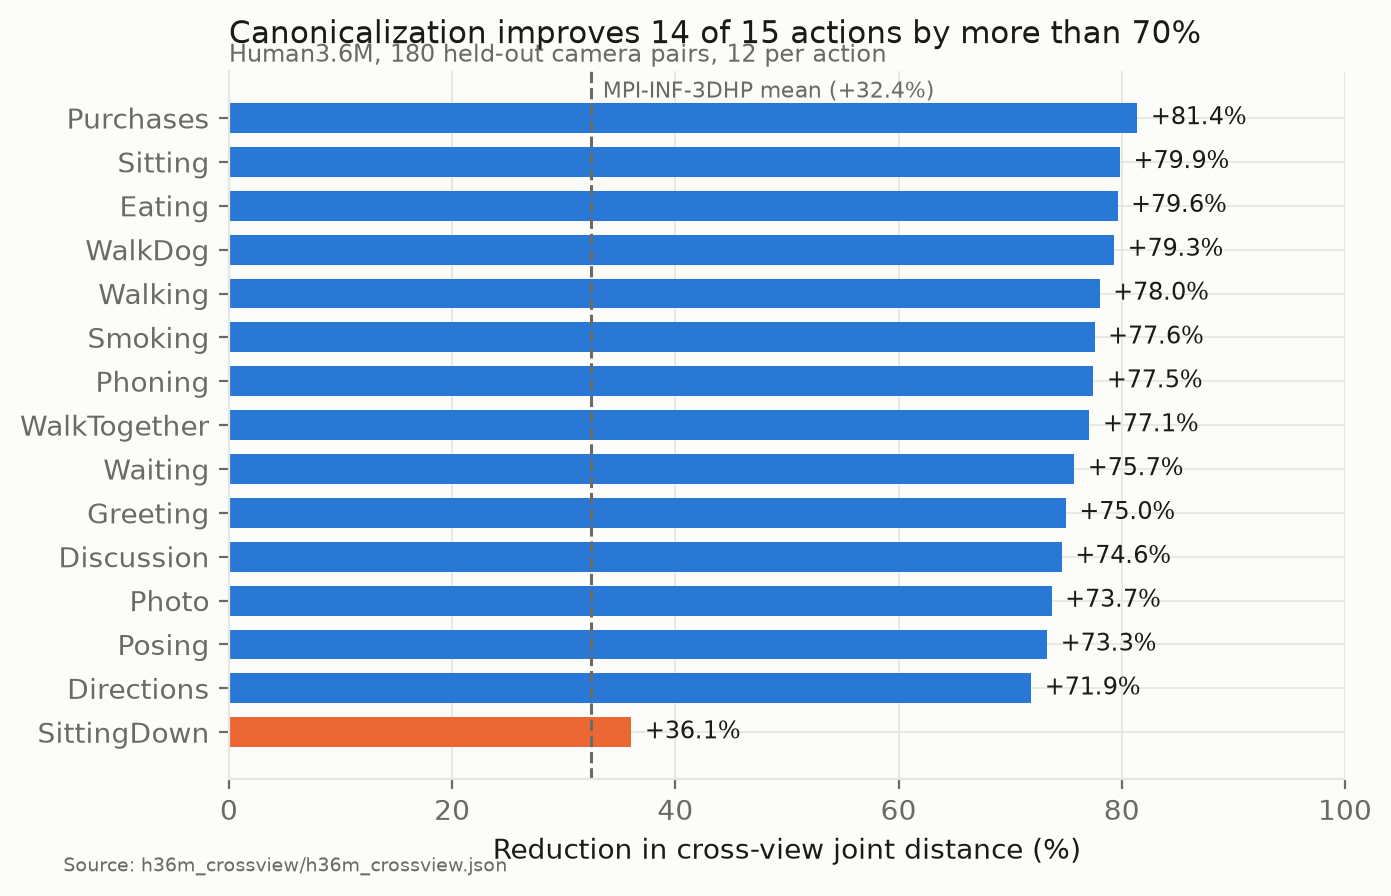
\includegraphics[width=0.92\textwidth]{images/fig_h36m_actions.png}
\caption[Per-action improvement on Human3.6M]{Per-action improvement on Human3.6M. Every action except SittingDown exceeds the mean improvement obtained on MPI-INF-3DHP by more than a factor of two.}
\label{fig:h36macts}
\end{figure}

The single exception is informative rather than embarrassing. All twelve SittingDown pairs carry a mean canonical distance of 274.1 mm, far above every other action, and SittingDown contains the one pair in 180 that regresses. SittingDown is also the action on which the backbone itself is least accurate, at 66.4 mm against a mean of 45.1 mm across actions. The body frame is constructed from the predicted torso and hip axes, so a pose the backbone estimates badly yields a frame estimated badly, and the error compounds rather than cancels.

We tested the competing explanation and rejected it. A seated subject might plausibly foreshorten the pelvis and leave the hip axis too short to define a stable frame, which is what we first supposed. Measured across the fifteen actions, the hip axis of SittingDown is 285.3 mm, the second longest of any action, while the shortest belongs to WalkDog at 268.4 mm, which canonicalizes at 79.3 percent without difficulty. The angle between the hip and torso axes is 86.0 degrees for SittingDown, inside the 83 to 88 degree band spanned by every action, so the frame is not ill-conditioned. Neither the length nor the conditioning of the axes distinguishes this action; only the accuracy of the pose they are built from does. Figure \ref{fig:h36msit} puts both candidate explanations on the same axes. Canonical distance is uncorrelated with hip-axis length across the fifteen actions, at $-0.03$, and correlates with the backbone's own accuracy at $+0.76$. That second association survives deleting SittingDown itself, at $+0.70$ over the remaining fourteen actions, so it describes a trend across actions rather than the influence of one outlier.

The failure is therefore inherited from the estimator rather than produced by the frame. This is a sharper statement than the one we began with and a less comfortable one, since a better frame construction cannot repair it.

\begin{figure}[htbp]
\centering
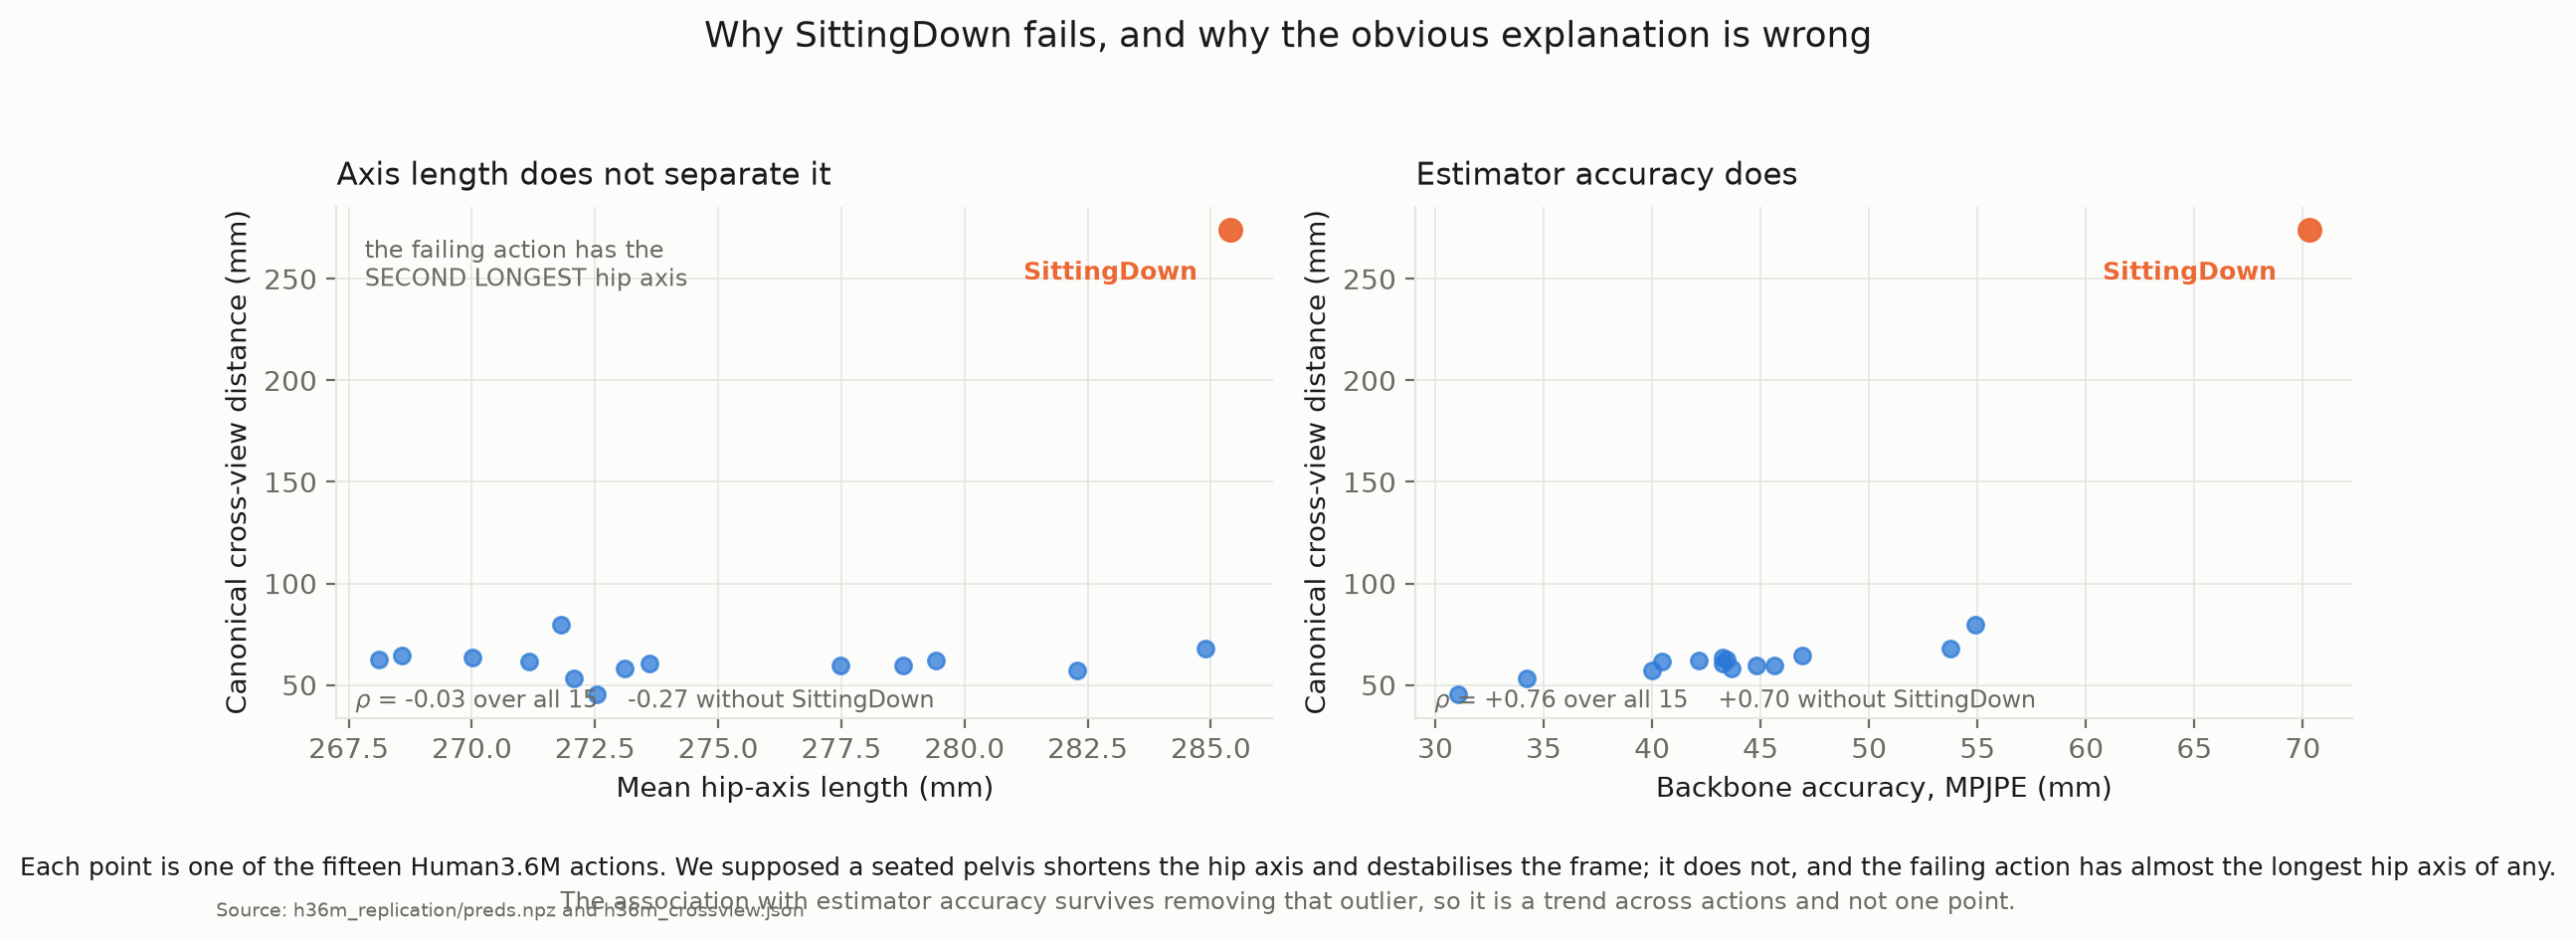
\includegraphics[width=\textwidth]{images/fig_h36m_sittingdown.png}
\caption[Two candidate explanations for the SittingDown result]{Two candidate explanations for the SittingDown result, tested against the fifteen actions. Axis length does not separate the failing action, which has almost the longest hip axis of any. Estimator accuracy does, and the association holds when the failing action is removed.}
\label{fig:h36msit}
\end{figure} The regressing pair additionally had an unusually small raw distance of 218.4 mm against roughly 550 mm for the other pairs of that action, which left little to gain and much to lose. That is the near-aligned camera pair behaviour reported on MPI-INF-3DHP in Section \ref{sec:crossview}, now observed on a second dataset.

We draw one further observation from placing this section beside Section \ref{sec:h36m}. The bone-length signal failed on Human3.6M because the backbone is accurate there, and canonicalization succeeds on Human3.6M for the same reason. Both depend on the quality of the predicted skeleton, and they depend on it in opposite directions.

\section{Multi-Scale Per-Limb Canonicalization on Human3.6M}
\label{sec:h36mms}

The multi-scale extension is the third component to receive the cross-dataset treatment. We compare the combined per-limb distance against the global frame on the same 180 held-out pairs, taking both quantities from the same code path so that the baseline and the treatment differ only in the frame used.

The extension replicates. Multi-scale reduces the combined cross-view distance from 62.7 mm to 46.2 mm,\footnote{The global frame appears here at 62.7 mm against the 75.3 mm of Section \ref{sec:h36mcv}, on the same 180 pairs and the same prediction cache. The two are not the same measurement. The cross-view experiment threads the previous frame's forward axis through the sequence for temporal sign consistency; the multi-scale module does not, and it computes its baseline and its treatment through that same unthreaded path so that the comparison is internally consistent by construction. Mixing them would score a threaded baseline against an unthreaded treatment and credit the difference to multi-scale. The absolute values in this section are therefore not comparable with those of Section \ref{sec:h36mcv}; the ratio between them is what this section reports.} an improvement of 25.6 percent with a cluster bootstrap interval of $[+23.6, +27.6]$ percent, and improves 179 of the 180 pairs. No segment fell back to the global frame on any evaluated pose, so the per-limb frames are well conditioned throughout. The improvement is largest exactly where the global frame is weakest: SittingDown gains 32.9 percent on all twelve of its pairs, against 17.8 percent for Walking. This is the expected relationship, since a limb frame is built from that limb's own joints and does not inherit the error in the torso and hip axes that Section \ref{sec:h36mcv} identified as the cause of the SittingDown result.

\subsection{A Bilateral Asymmetry, and What Caused It}

The per-level breakdown revealed a defect in our own implementation that the MPI-INF-3DHP evaluation had not exposed. The two arms agree closely, at 57.1 mm and 57.6 mm, which is what bilateral symmetry predicts for a subject performing symmetric everyday actions. The two legs do not: the right leg scores 69.4 mm against 30.7 mm for the left, a factor of 2.3. We note that the segment keys in our implementation are mirrored with respect to anatomy, so the key named \texttt{left\_leg} holds the joints of the anatomical right leg. Anatomical names are used throughout this section and in Table \ref{tab:msfix}; the mirroring affects labels only and no geometry or number depends on it.

Inspecting the segment definitions explains it. Both arms take the thorax-to-shoulder vector as primary axis and the shoulder-to-elbow vector as secondary. The legs were defined inconsistently with each other: the left leg takes hip-to-knee as primary and knee-to-ankle as secondary, while the right leg takes root-to-hip as primary and hip-to-knee as secondary. The root-to-hip vector is roughly half a hip width, whereas hip-to-knee is a full thigh. Section 3.2 argues that frame sensitivity to joint error scales inversely with the length of the defining vector, so the right leg was predicted to be the noisier of the two before the cause was found, and for exactly this reason.

We tested the correction rather than assuming it. Defining both legs identically, with hip-to-knee as primary and knee-to-ankle as secondary, gives the middle column of Table \ref{tab:msfix}. The right leg falls from 69.4 mm to 29.3 mm, which brings it into agreement with the left leg at 30.7 mm. Every other level is unchanged to the reported precision, which is the signature of a correct diagnosis rather than a general perturbation. The combined distance falls from 46.2 mm to 39.1 mm, the improvement over the global frame rises from 25.6 percent to 37.2 percent, and all 180 pairs now improve rather than 179.

\subsection{The Same Defect in Both Arms}

Applying the diagnosis consistently exposes a second instance of it. Both arms take the thorax-to-shoulder vector as primary axis, which is about half a shoulder width, where the corrected legs take a full thigh. The bilateral comparison could not reveal this, because both arms share the defect and therefore agree with each other at 57.1 mm and 57.6 mm. Agreement between two measurements is not evidence that either is correct, and here it actively concealed the problem: the arms looked healthy precisely because they were equally affected.

Rebuilding both arms from their own long segments, shoulder-to-elbow as primary and elbow-to-wrist as secondary, produces the largest single improvement in this chapter. The right arm falls from 57.1 mm to 26.8 mm and the left from 57.6 mm to 26.3 mm. The combined multi-scale distance falls to 28.2 mm, the improvement over the global frame reaches 55.1 percent with a cluster bootstrap interval of $[+53.6, +56.5]$ percent, and all 180 pairs improve with no segment falling back to the global frame.

The corrected levels support the diagnosis independently of the improvement they produce. All five now lie between 26.3 mm and 30.7 mm, where before they ranged from 28.6 mm to 69.4 mm. A construction applied consistently to five anatomically different segments should give five similar numbers, and it now does. That convergence was not optimized for, since each segment was redefined by the same rule rather than tuned.

An earlier version of this report called that convergence the strongest evidence that axis length, not anatomy, was driving the spread. \textbf{Section \ref{sec:circularity} withdraws that reading.} Every one of these five levels is built entirely or mostly from the joints it is then scored on --- the four limbs from three of three, the torso from four of six --- and convergence into a narrow band is what that circularity predicts on its own, without any contribution from axis length. The convergence is therefore reported here as a consistency check on the implementation fix, confirming that one rule was applied uniformly, and not as evidence for the axis-length principle. The evidence for that principle is the global-frame comparison of Section \ref{sec:multilandmark}, where the scored set and the constructor count are held identical and only the axis length differs.

\begin{table}[htbp]
\centering
\caption[Building every segment frame from that segment's own long axis]{Building every segment frame from that segment's own long axis. Bold entries changed from the column to their left.}
\label{tab:msfix}
\begin{tabular}{lrrr}
\hline
\textbf{Level} & \textbf{As implemented} & \textbf{Legs alike} & \textbf{Arms also} \\
\hline
Global frame & 62.7 mm & 62.7 mm & 62.7 mm \\
Torso & 28.6 mm & 28.6 mm & 28.6 mm \\
Right arm & 57.1 mm & 57.1 mm & \textbf{26.8 mm} \\
Left arm & 57.6 mm & 57.6 mm & \textbf{26.3 mm} \\
Right leg & 69.4 mm & \textbf{29.3 mm} & 29.3 mm \\
Left leg & 30.7 mm & 30.7 mm & 30.7 mm \\
\hline
Combined multi-scale & 46.2 mm & \textbf{39.1 mm} & \textbf{28.2 mm} \\
Improvement over global & +25.6\% & \textbf{+37.2\%} & \textbf{+55.1\%} \\
95\% CI & $[+23.6, +27.6]$ & --- & $\mathbf{[+53.6, +56.5]}$ \\
Pairs improved & 179 / 180 & \textbf{180 / 180} & \textbf{180 / 180} \\
\hline
\end{tabular}
\end{table}

\begin{figure}[htbp]
\centering
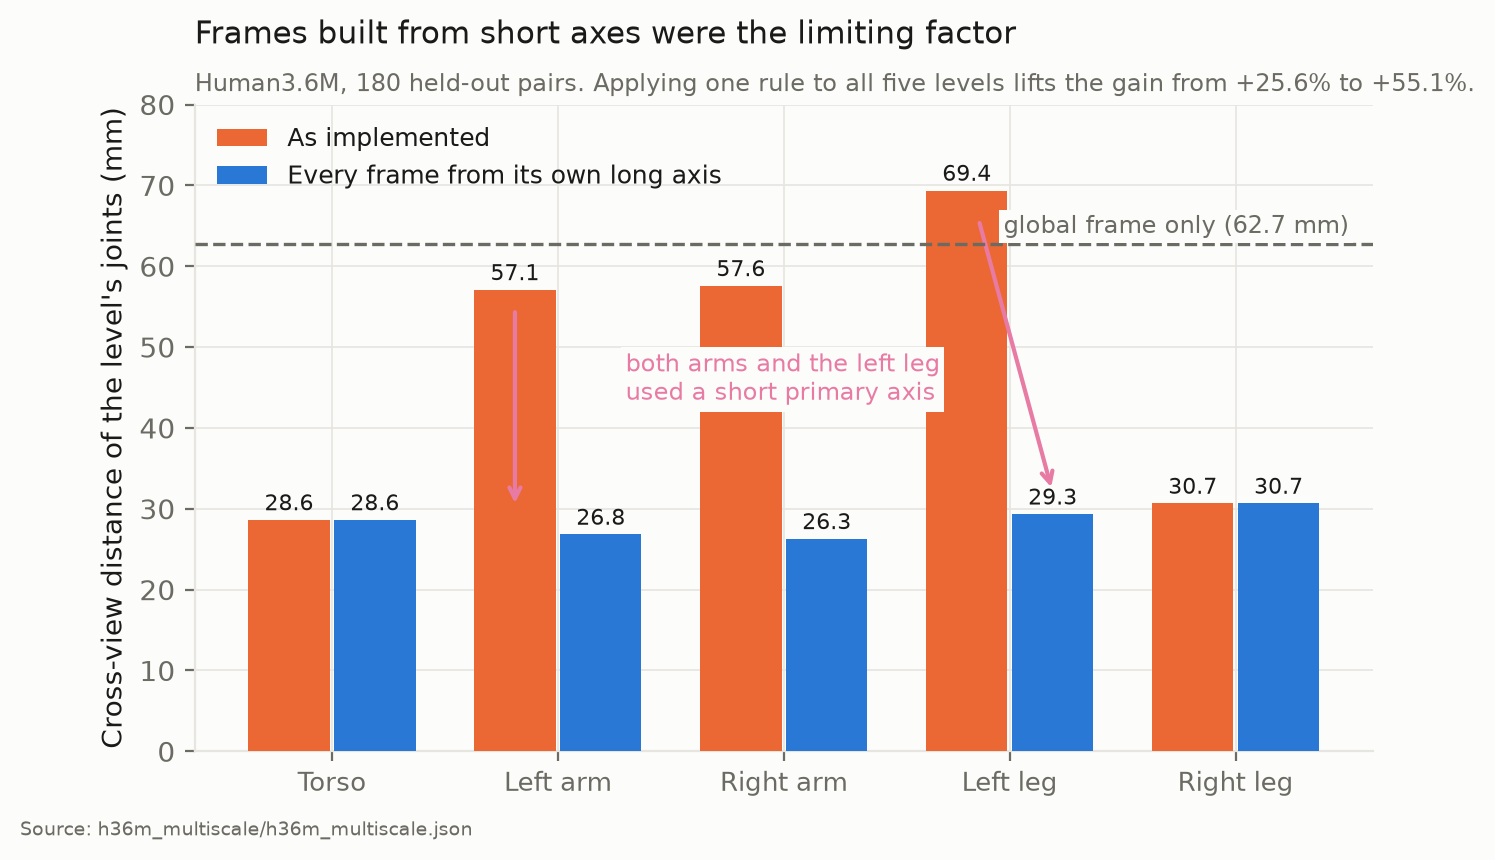
\includegraphics[width=0.97\textwidth]{images/fig_h36m_multiscale.png}
\caption[Per-level cross-view distance on Human3.6M]{Per-level cross-view distance on Human3.6M. Three of the five frames were built from an axis roughly half a shoulder or hip width long; rebuilding them from the segment's own long axis halves their cross-view distance and brings all five levels into a 4.4 mm band.}
\label{fig:h36mms}
\end{figure}

Two remarks are in order. The first concerns what the correction is not: it adds no parameters, consumes no labels and changes no algorithm, since it only makes two segment definitions agree with each other and with the four that were already consistent. The second concerns why it went unnoticed. The MPI-INF-3DHP evaluation reported one combined number per camera pair and confirmed that multi-scale beat the global frame, which it did. The defect was invisible at that granularity and became obvious only when the levels were reported separately on a dataset large enough for the bilateral comparison to be unambiguous. We report the corrected figures as a variant rather than as the headline, because the MPI-INF-3DHP results elsewhere in this chapter were produced with the original definitions and we have not re-run them.

\section{Ablation with Abstention}

Table \ref{tab:ablation} reports the three conditions on the development pair and Figure \ref{fig:coverage} traces error against coverage as the abstention threshold varies. Coverage is reported alongside error throughout, since an abstaining method could otherwise report an arbitrarily low error by answering arbitrarily rarely.

\begin{table}[htbp]
\centering
\caption{Three conditions on the development pair}
\label{tab:ablation}
\begin{tabular}{|l|c|c|}
\hline
\textbf{Condition} & \textbf{Distance} & \textbf{Coverage} \\
\hline
Raw root-relative & 0.1439 & 100\% \\
\hline
Canonical & 0.1143 & 100\% \\
\hline
Reliability-aware, threshold 0.5 & 0.1044 & 89\% \\
\hline
Reliability-aware, threshold 0.8 & \textbf{0.0904} & 69\% \\
\hline
\end{tabular}
\end{table}

\begin{figure}[htbp]
\centering
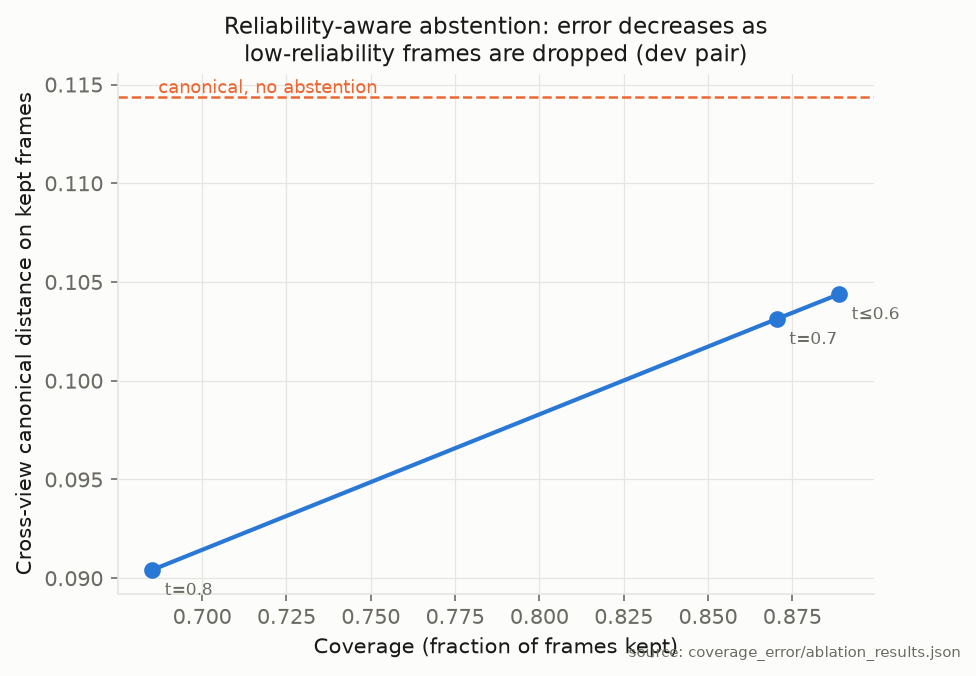
\includegraphics[width=0.68\textwidth]{images/fig_coverage_error.png}
\caption{Coverage against error as the abstention threshold varies}
\label{fig:coverage}
\end{figure}

\section{Negative Result on Cross-View Retrieval}
\label{sec:retrieval}

Canonicalization degrades cross-view retrieval, with recall at rank one falling from 0.02 to 0.00 and mean reciprocal rank falling by 6.9 percent. This outcome is consistent with expectation, because retrieval across similar standing poses relies in part on viewpoint information, which canonicalization removes by construction.

We flag one limitation of this experiment explicitly, because it is a departure from the protocol used everywhere else in this report. It predates the correction described in Section \ref{sec:protocol}: it evaluates fifty near-identical standing poses under the superseded single-frame protocol, and a recall at rank one of 0.02 before canonicalization indicates that the task was close to chance to begin with, so there was little for the method to degrade. We therefore report the number as a bound rather than as a measurement, and we do not claim it establishes that canonicalization harms retrieval in general. A proper test would use the cached Human3.6M predictions and a gallery drawn per subject and action, and it is listed in Section \ref{sec:future} as future work rather than presented here.

% ========================== CHAPTER 5 ================================
